\section{Klassifikatoren}
Bei der Entwicklung des Prototyps zur Klassifikation von Schüttgut wurde ein Ansatz verfolgt, der den einfachen Austausch des Klassifikators erlaubt. In der Folge konnten mehrere verschiedene Klassifikatoren getestet und verglichen werden. In Kapitel 3.1 wird ein Naive Bayes Klassifikator beschrieben und in Kapitel 3.2 ein k-Nearest Neighbour Klassifikator. Für die beiden vielversprechendsten Klassifikatoren Boosted Decision Trees (vgl. Kapitel 3.3) und Neuronal Networks (vgl. Kapitel 3.4) wurden sowohl das Lernverfahren, als auch die Parameter der Klassifikatoren optimiert.

\subsection{Naive Bayes}
Da der bestehende Naive Bayes Klassifikator (MA) nicht ohne weiteres in unseren Prototyp integriert werden konnte, haben wir einen eigenen Bayes Klassifikator erstellt. Die Ergebnisse dieses Klassifikators stellen die Referenzwerte dar, mit denen wir unsere optimierten Klassifikatoren vergleichen.

Der Bayes Klassifikator erhält die zuvor berechnete Featuretabelle (vgl. Kapitel 4) von zwei unterschiedlichen Klassen von Schuettgut als Eingabe und klassifiziert die Teilchen in zwei Schritten. Im Trainingsschritt werden anhand der Trainingsdaten die Parameter der Wahrscheinlichkeitsverteilung geschätzt. Im Vorhersageschritt werden die Teilchen der Testdaten anhand ihrer a posteriori Wahrscheinlichkeit einer Schüttgutklasse zugeordnet. ( https://de.mathworks.com/help/stats/naive-bayes-classification.html )


\subsection{k-Nearest Neighbors}

\subsection{Boosted Decision Trees}

\subsection{Neural Network}

Aufbau des Netzes
Input
Hidden Layers
Output

\begin{figure}[!h]
    \centering
    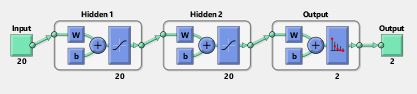
\includegraphics[width=1\textwidth]{pics/NN-Structure.JPG}
    \caption{Struktur des Neuronalen Netzes}
    \label{fig:NNStructure}
\end{figure}

\subsubsection{Lernverfahren}
Levenberg-Marquardt backpropagation

Methode der kleinsten Quadrate
kombiniert Gauß-Newton-Verfahren mit Regularisierungstechnik
robust, konvergiert auch bei schlechten Startbedingungen
Konvergenz nicht garantiert
langsam bei Anfangswerten nahe Minimum

Bayesian regularization backpropagation

Benutzt auch Levenberg-Marquardt
in Matlab: Benötigt länger (alle Epochen), aber z.T. deutlich bessere Ergebnisse (bspw. Feature VelocitiesAfterPositionNew(10) F1Score: +0.81212 (trainlm) vs. F1Score: +0.94297 (trainbr)
robuster
kaum overfitting und overtraining
calculates and trains on a number of effective network parameters or weights, effectively turning off those that are not relevant. This effective number is usually considerably smaller than the number of weights in a standard fully connected back-propagation neural net.
Scaled conjugate gradient backpropagation

Resilient backpropagation
